\documentclass{beamer}
\author[Murphy]{Francisco Murphy Pérez\inst{1}}
\institute{1: UNAM-IBt.}
\date{francisco.murphy@ibt.unam.mx\\19 julio 2023}
\title{Curso propedéutico de química}
\subtitle{UAEM-CIDC}
\usetheme[progressbar=frametitle,numbering=fraction,block=fill,background=light]{metropolis}
% Carga algunos paquetes.
\usepackage[spanish,mexico]{babel} %T raduce a español mexicano, por favor.
\usepackage{booktabs} % Las tablas se ven más pro'.
\usepackage{siunitx} % Permite usar números-unidades de manera coherente.
\usepackage{chemformula} % Para fórmulas químicas.
\usepackage{elements} % Para configuración electrónica.
\usepackage{chemfig} % Para fórmulas estructurales. 
\setchemfig{compound sep=7em, arrow offset=2em, + sep left=1.5em, + sep right=1.5em}
\setcharge{.radius=0.2ex}
\usepackage{bohr} % Para dibujra el átomo de Bohr.
\usepackage{chemmacros} % Necesario para que las cargas dentro de los átomos de Bohr se hagan pequeñas.
% Las siguientes tres líneas hacen un handout. Descomentarlas, si quiere un handout.
%\usepackage{pgfpages}
%\pgfpagesuselayout{resize to}[a4paper, border shrink=1mm,landscape]
%\pgfpagesuselayout{4 on 1}[a4paper, border shrink=1mm,landscape]
\begin{document}
  \begin{frame}
    \titlepage
  \end{frame}
  %%%%%%%%%%%%%%%%%%%%%%%%%%%%%%%%%%%%%%%%%%%%%%%%%%%%%%%%%%%%
  \section{Recordando...}
  %%%%%%%%%%%%%%%%%%%%%%%%%%%%%%%%%%%%%%%%%%%%%%%%%%%%%%%%%%%%
  \begin{frame}{Recordando...}
    \begin{table}[]
      \centering
      \resizebox{0.7\textwidth}{!}{%
        \begin{tabular}{@{}llll@{}}
          \toprule
          Partícula & Masa (\unit{\kilogram}) & Masa (u) & Carga \\ \midrule
          protón   & \num{1.67262e-27} & 1.0073  & 1+ \\
          neutrón  & \num{1.67493e-27} & 1.0087  & 0 \\
          electrón & \num{0.00091e-27} & 0.00055 & 1- \\ \bottomrule
        \end{tabular}%
      }
      \caption{Propiedades de partículas subatómicas.}
      \label{tab:my-table}
    \end{table}
  \end{frame}
  %%%%%%%%%%%%%%%%%%%%%%%%%%%%%%%%%%%%%%%%%%%%%%%%%%%%%%%%%%%%
  \begin{frame}{Recordando...}
    % Por acuerdo internacional, 
    Una unidad de masa atómica (antes uma, ahora u) se define como una masa exactamente igual a una doceava parte de la masa de un átomo de carbono-12.\par
    % Una unidad de masa atómica también se conoce como un Dalton, llamado así por John Dalton. El carbono-12 es el isótopo de carbono que tiene seis protones y seis neutrones.
    Así es fácil comparar la masa atómica de los otros elementos. Por ejemplo, en promedio, un átomo de hidrógeno tiene \qty{8.4}{\percent} la masa del átomo de carbono-12. Por lo tanto, la masa atómica del hidrógeno debe ser \(0.084\cdot\qty{12}{\,\text{u}} = \qty{1.008}{\,\text{u}} \).
    % 1 uma = 1.661X10-24 g
  \end{frame}
  %%%%%%%%%%%%%%%%%%%%%%%%%%%%%%%%%%%%%%%%%%%%%%%%%%%%%%%%%%%%
  \begin{frame}{Recordando...}
    \begin{figure}
      \centering
      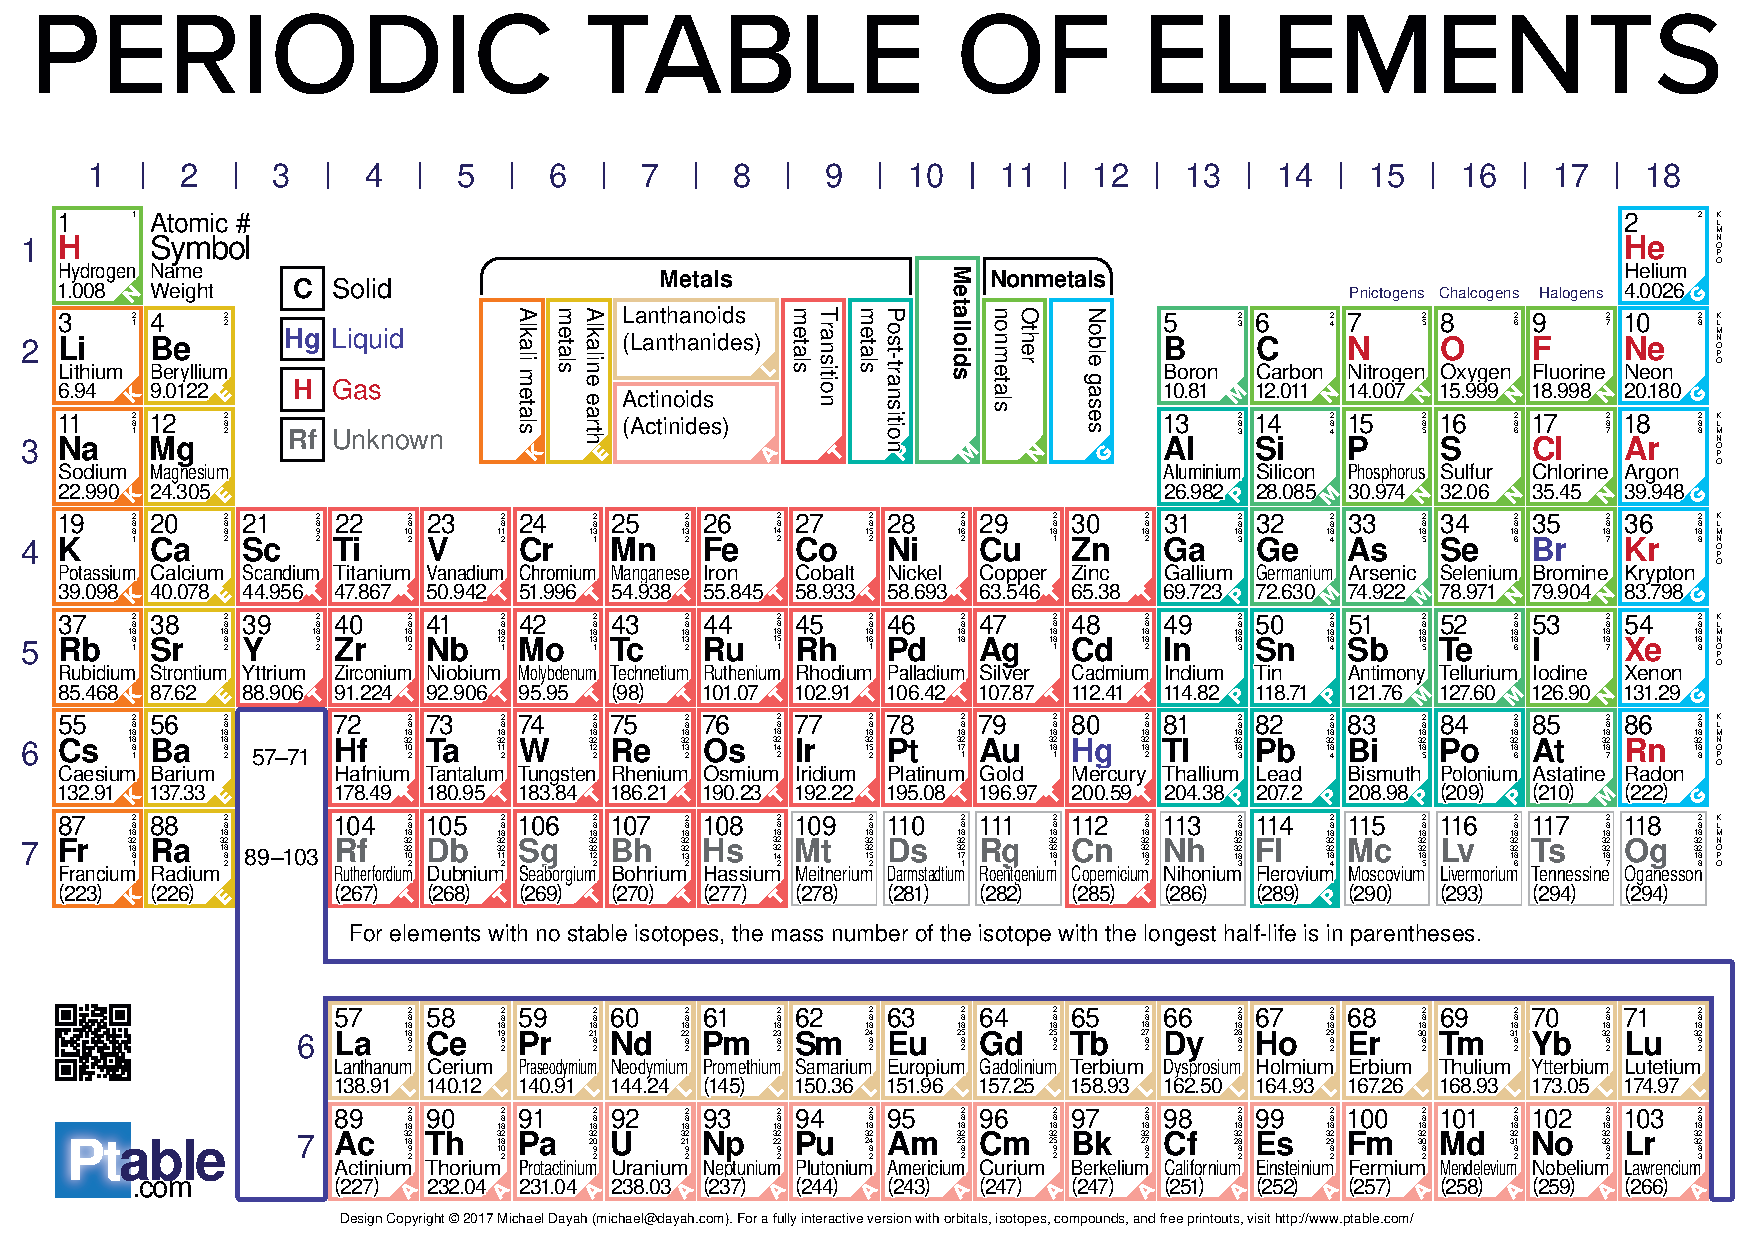
\includegraphics[width=0.9\linewidth]{imgs/periodic-table.pdf}
      \caption{Tabla periódica de los elementos. Fuente: \href{https://ptable.com}{ptable.com}.}
      % Preguntarles:
      % Cómo está ordenada la tabla periódica?
      % Qué significa la masa atómica? 
      % Por qué el carbono en la tabla periódica no es 12 u exactamente? (según nuestra definición).
      \label{fig:pt-atomic-mass}
    \end{figure}
  \end{frame}
  %%%%%%%%%%%%%%%%%%%%%%%%%%%%%%%%%%%%%%%%%%%%%%%%%%%%%%%%%%%%
  \begin{frame}{Recordando...}
    La masa atómica es un promedio ponderado. Por ejemplo:
    \begin{itemize}
      \item \qty{75.77}{\percent} cloro-35, \qty{24.23}{\percent} cloro-37; con una masa atómica de \num{34.97} y \qty{36.97}{u}, respectivamente.
      \[(0.7577\cdot\qty{34.97}{u}) + (0.2423\cdot\qty{36.97}{u}) = \qty{35.45}{u}\]
      % Otro ejemplo que no cabe :P
      %\item \qty{98.90}{\percent} carbono-12, \qty{1.10}{\percent} carbono-13; con una masa atómica de \num{12} y \qty{13.00335}{u}.
    \end{itemize}
    \begin{block}{Cuidado:}
      De cien veces que pesemos la masa de un átomo de cloro, 76 veces su masa será \qty{34.97}{u} y 24 veces su masa será \qty{36.97}{u}. Nunca saldrá una masa de \qty{35.45}{u}.
    \end{block}
  \end{frame}
  %%%%%%%%%%%%%%%%%%%%%%%%%%%%%%%%%%%%%%%%%%%%%%%%%%%%%%%%%%%%
  \begin{frame}{Recordando...}
    \begin{block}{Una molécula...}
      es un agregado de, por lo menos, dos átomos en un arreglo definido que se mantienen unidos a través de enlaces químicos.
    \end{block}
    % Una molécula puede contener átomos del mismo elemento o átomos de dos o más elementos, siempre en una proporción fija.
    \begin{block}{Un ión...}
      es un átomo (o un grupo de átomos) que tiene(n) una carga neta positiva o negativa.
    \end{block}
    % Preguntarles:
    % Cómo se forma un ión? 
  \end{frame}
  %%%%%%%%%%%%%%%%%%%%%%%%%%%%%%%%%%%%%%%%%%%%%%%%%%%%%%%%%%%%
  \begin{frame}{Recordando...}
    \begin{itemize}
      \item Sustancias puras
      \begin{itemize}
        \item Elementos
        \begin{itemize}
          \item Atómicos (\ch{He}, \ch{Ne}, \ch{Cu}, \ch{Hg})
          \item Moleculares (\ch{O2}, \ch{H2}, \ch{Cl2}, \ch{Br2})
        \end{itemize}
        \item Compuestos
        \begin{itemize}
          \item Moleculares (\ch{H2O}, \ch{CO2}, \ch{(CH3)2CO})
          \item Iónicos (\ch{NaCl}, \ch{KBr}, \ch{LiF})
        \end{itemize}
      \end{itemize}
    \end{itemize}
  \end{frame}
  %%%%%%%%%%%%%%%%%%%%%%%%%%%%%%%%%%%%%%%%%%%%%%%%%%%%%%%%%%%%
  \section{Fórmulas y Moles}
  %%%%%%%%%%%%%%%%%%%%%%%%%%%%%%%%%%%%%%%%%%%%%%%%%%%%%%%%%%%%
  \begin{frame}{Fórmulas químicas}
    Sirven para expresar la composición de las moléculas y los compuestos iónicos por medio de los símbolos químicos.\par 
    \emph{Composición} significa, qué átomos hay presentes y en qué proporción...\par
    Tres tipos de fórmulas:
    \begin{itemize}
      \item empíricas
      \item moleculares
      \item estructurales
    \end{itemize}
  \end{frame}
  %%%%%%%%%%%%%%%%%%%%%%%%%%%%%%%%%%%%%%%%%%%%%%%%%%%%%%%%%%%%
  \begin{frame}{Fórmula molecular}
    Indica el número exacto de átomos, de cada elemento, presentes en la unidad más pequeña de una sustancia. Por ejemplo:
    \begin{itemize}
      \item \ch{H2O} monóxido de dihidrógeno\footnote{\href{https://en.wikipedia.org/wiki/Dihydrogen_monoxide_parody}{Dato curioso}.} (agua)
      \item \ch{H2} hidrógeno molecular
      \item \ch{NaCl} cloruro de sodio\footnote{Los compuestos iónicos no están formados por moléculas. Estrictamente hablando, se dice \emph{unidad de fórmula}  en vez de \emph{fórmula molecular} para un compuesto iónico.}
      \item \ch{O2} oxígeno molecular
      \item \ch{CH4} metano
      \item \ch{O3} ozono
    \end{itemize} 
  \end{frame}
  %%%%%%%%%%%%%%%%%%%%%%%%%%%%%%%%%%%%%%%%%%%%%%%%%%%%%%%%%%%%
  \begin{frame}{Masa molecular}
    La suma de las masas atómicas de cada átomo en una molécula. 
    Por ejemplo:
    \begin{align*}
      \ch{H2O}&: 2(1.01 \,\text{u}) + 1(16.00\,\text{u})  = 18.02 \,\text{u} \\
      \ch{NaCl}&: 1(22.99 \,\text{u}) + 1(35.45 \,\text{u}) = 58.44 \,\text{u} \\
      \ch{C6H12O6}&: 6(12.01 \,\text{u}) + 12(1.01 \,\text{u}) + 6(16.00 \,\text{u}) = 180.16 \,\text{u}
    \end{align*}
  \end{frame}
  %%%%%%%%%%%%%%%%%%%%%%%%%%%%%%%%%%%%%%%%%%%%%%%%%%%%%%%%%%%%
  \begin{frame}{Ejercicios:}
    Calcular la masa molecular de:
    \begin{columns}
      \column{0.5\textwidth}
      \begin{align*}
        \ch{NO2}\quad & \only<1>{\line(1,0){50}} & \only<2>{\qty{46.01}{u}}\\
        \ch{Li2SO4}\quad & \only<1>{\line(1,0){50}} & \only<2>{\qty{109.94}{u}}\\
        \ch{Al2O3}\quad & \only<1>{\line(1,0){50}} & \only<2>{\qty{101.96}{u}}\\
        \ch{Fe2S3}\quad & \only<1>{\line(1,0){50}} & \only<2>{\qty{207.89}{u}}  
      \end{align*}
      \column{0.5\textwidth}
      \begin{align*}
        \ch{Co(ClO4)2}\quad & \only<1>{\line(1,0){50}} & \only<2>{\qty{257.83}{u}}\\
        \ch{C6H12O6}\quad & \only<1>{\line(1,0){50}} & \only<2>{\qty{180.16}{u}}\\
        \ch{C2H5NO2}\quad & \only<1>{\line(1,0){50}} & \only<2>{\qty{75.07}{u}}\\
        \ch{C10H16N5O13P3}\quad & \only<1>{\line(1,0){50}} & \only<2>{\qty{507.18}{u}}
      \end{align*}
    \end{columns}
  \end{frame}
  %%%%%%%%%%%%%%%%%%%%%%%%%%%%%%%%%%%%%%%%%%%%%%%%%%%%%%%%%%%%
  \begin{frame}{Mol}
    Similar a: 
    \begin{itemize}
      \item un par (dos objetos)
      \item una docena (doce objetos)
      \item una gruesa (144 objetos)
    \end{itemize}
    Un mol contiene \qty{6.022e23}{\text{objetos}}\footnote{Objetos en este contexto significa átomos, moléculas, electrones, iones, partículas alfa, etc.}. Este número se conoce como el número de Avogadro (\(N_{\mathrm{A}}\)).\par
    Anteriormente un mol se definía igual al número de átomos en exactamente 12 g de carbono-12. (vea \href{https://en.wikipedia.org/wiki/Mole_(unit)\#Standardization}{aquí})
    % Objetos puede ser lo que sea... barras de chocolate, estrellas, canicas. Pero la cuestión es que es un número muuuy grande, para contar cosas muuuy pequeñas. Un mol de canicas llenaría la tierra significa más canicas que estrellas.
  \end{frame}
  %%%%%%%%%%%%%%%%%%%%%%%%%%%%%%%%%%%%%%%%%%%%%%%%%%%%%%%%%%%%
  \begin{frame}{Masa molar}
    %The value of an element’s molar mass in grams per mole is numerically equal to the element’s atomic mass in atomic mass units.
    La masa de un mol de átomos de un elemento\footnote{Recuerde que el valor numérico en masa molar (\unit{\gram\per\mole}) es igual a la masa atómica (\unit{u}). Las unidades son diferentes.}.
    \begin{figure}
      \centering
      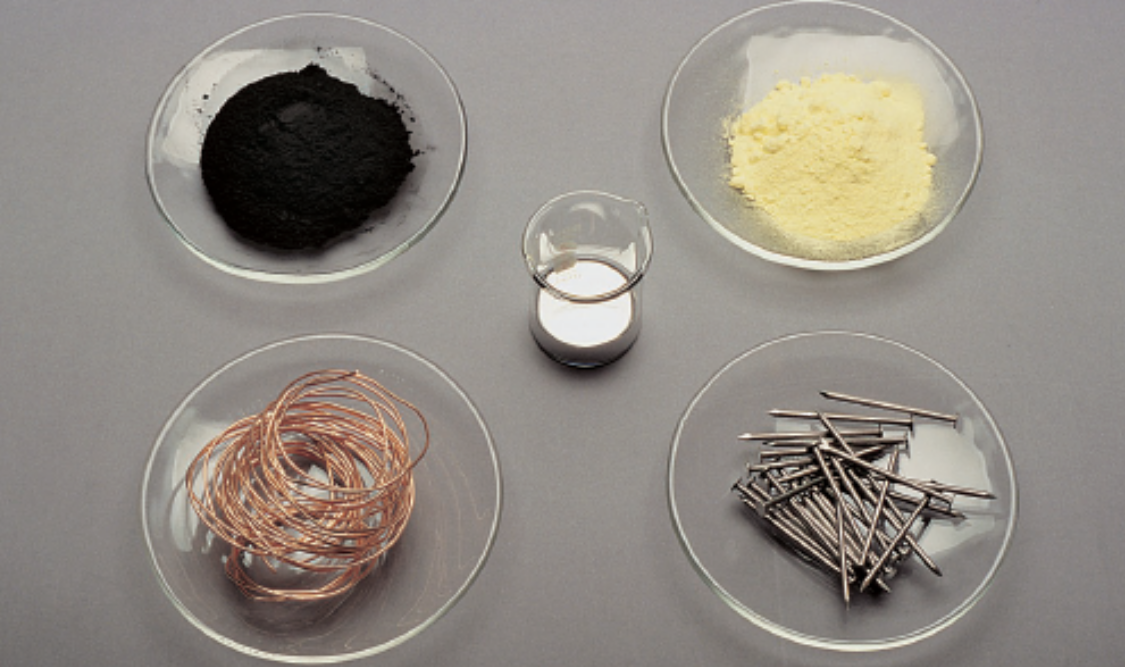
\includegraphics[width=0.7\linewidth]{imgs/mol}
      \caption{Un mol de: carbono, azufre, cobre, hierro y mercurio. Fuente: Chemistry, decimocuarta edición, R. Chang \& J. Overby. }
      \label{fig:mol}
    \end{figure}
  \end{frame}
  %%%%%%%%%%%%%%%%%%%%%%%%%%%%%%%%%%%%%%%%%%%%%%%%%%%%%%%%%%%%
  \begin{frame}{Conversiones}
    Los conceptos anteriores permiten efectuar conversiones entre masa, moles y número de objetos (átomos, iones, moléculas, etc). Por ejemplo; calcular el número de átomos de carbono en \qty{0.58}{\gram} de carbono:\par
    \begin{align*}
      & \qty{0.58}{\gram\,C}\cdot\left[\frac{\qty{1}{\mole\,C}}{\qty{12.01}{\gram\, C}}\right]\cdot\left[\frac{\qty{6.022e23}{\text{átomos de C}}}{\qty{1}{\mole\,C}}\right]=\\[5pt] \onslide<2>{&\qty{2.91e22}{\text{átomos de C}}}
    \end{align*}
  \end{frame}
  %%%%%%%%%%%%%%%%%%%%%%%%%%%%%%%%%%%%%%%%%%%%%%%%%%%%%%%%%%%%
  \begin{frame}{Ejercicios:}
    Cuánto pesa un átomo de carbono-12?
    \onslide<2>{\[\left[\frac{\qty{12.01}{\gram\,C}}{\qty{1}{\mole\,C}}\right]\cdot\left[\frac{\qty{1}{\mole\,C}}{\qty{6.022e23}{\text{átomos de C}}}\right]=\qty{2e-23}{\gram\per\text{átomo de C}}\]}
    Cuánta masa (en g) hay en \qty{2.5}{\mole} de agua?
    \onslide<2>{\[\qty{2.5}{\mole\,\ch{H2O}}\cdot\left[\frac{\qty{18.02}{\gram\,\ch{H2O}}}{\qty{1}{\mole\,\ch{H2O}}}\right]=\qty{45.05}{\gram\,\ch{H2O}}\]}
    Cuántos átomos de helio hay en \qty{6.46}{\gram} de helio?
    \onslide<2>{
      \begin{align*}
        & \qty{6.46}{\gram\,He}\cdot \left[\frac{\qty{1}{\mole\,He}}{\qty{4.003}{\gram\,He}}\right]\cdot\left[\frac{\qty{6.022e23}{\text{átomos de He}}}{\qty{1}{\mole\,He}}\right]=\\[5pt]
        & \qty{9.7e23}{\text{átomos de He}}
      \end{align*}}
  \end{frame}
  %%%%%%%%%%%%%%%%%%%%%%%%%%%%%%%%%%%%%%%%%%%%%%%%%%%%%%%%%%%%
  \begin{frame}{Composición porcentual de masa}
    O simplemente porcentaje de masa de un elemento, es el porcentaje del elemento de la masa total del compuesto. Por ejemplo; calcular el porcentaje de masa de \ch{Cl} de la molécula \ch{CCl2F2}:\par
    \begin{align*}
      %&\ch{CCl2F2}: 1(12.01) + 2(35.45) + 2(19.00) = \qty{120.91}{\gram\per\mole} \\
      %&\text{Si} \quad\qty{120.91}{\gram\per\mole} \rightarrow \quad\qty{100}{\percent}\\
      %&\text{Entonces...} \\
      &\left[\frac{\qty{2}{\mole\,Cl}}{\qty{1}{\mole\,\ch{CCl2F2}}}\right]\cdot\left[\frac{\qty{1}{\mole\,\ch{CCl2F2}}}{\qty{120.91}{\gram\,\ch{CCl2F2}}}\right]\cdot\left[\frac{\qty{35.35}{\gram\,Cl}}{\qty{1}{\mole\,Cl}}\right]=\\[5pt]
      &\qty{0.586}{\gram\,Cl\per\gram\,\ch{CCl2F2}}
    \end{align*}
    Significa que se tiene \qty{0.586}{\gram} de \ch{Cl} por cada \unit{\gram} de \ch{CCl2F2}, o bien \qty{58.6}{\percent} de \ch{Cl} por \qty{100}{\percent} de \ch{CCl2F2}. 
  \end{frame}
  %%%%%%%%%%%%%%%%%%%%%%%%%%%%%%%%%%%%%%%%%%%%%%%%%%%%%%%%%%%%
  \begin{frame}{Fórmula empírica}
    Indica qué elementos están presentes y la proporción mínima entre sus átomos (en números enteros). No necesariamente indica el número real de átomos en una molécula dada\footnote{En general, la unidad de fórmula es la fórmula más simple para un compuesto iónico.}.\par
    Por ejemplo: la fórmula molecular \ch{H2O2}, fórmula empírica \ch{HO}.
    % Una vez que se conoce la fórmula molecular, también se sabe la fórmula empírica, pero no al contrario.
    % Las fórmulas de los compuestos iónicos por lo general son las mismas que sus fórmulas empíricas, debido a que los compuestos iónicos no están formados por unidades moleculares discretas.
  \end{frame}
  %%%%%%%%%%%%%%%%%%%%%%%%%%%%%%%%%%%%%%%%%%%%%%%%%%%%%%%%%%%%
  \begin{frame}{Ejercicios:}
    % Según la RAE, \emph{empírico}: perteneciente o relativo a la experiencia. 
    % Normalmente se descubre primero la fórmula empírica y luego la fórmula molecular.
    \only<1>{Una molécula se compone de \qty{40.92}{\percent} de \ch{C}, \qty{4.58}{\percent} de \ch{H} y \qty{54.5}{\percent} de \ch{O}. Determine su fórmula empírica.}
    \only<2>{Primero consiga moles:
        \begin{align*}
          \qty{40.92}{\gram\,C}&\cdot\left[\frac{\qty{1}{\mol}}{\qty{12.01}{\gram\,C}}\right]=\qty{3.407}{\mole\,C}\\
          \qty{4.58}{\gram\,H}&\cdot\left[\frac{\qty{1}{\mol}}{\qty{1.008}{\gram\,H}}\right]=\qty{4.54}{\mole\,H}\\
          \qty{54.50}{\gram\,O}&\cdot\left[\frac{\qty{1}{\mol}}{\qty{16.00}{\gram\,O}}\right]=\qty{3.406}{\mole\,O}
        \end{align*}}
      \only<3>{Luego determine la proporción entre los moles:
         \begin{align*}
          \frac{\qty{3.407}{\mole\,C}}{\qty{3.406}{\mole\,O}}&\approx\qty{1}{\mole\,C\per\mole\,O}\\[5pt]       \frac{\qty{4.58}{\mole\,H}}{\qty{3.406}{\mole\,O}}&\approx\qty{1.33}{\mole\,H\per\mole\,O}       %\frac{\qty{3.406}{\mole\,O}}{\qty{3.406}{\mole\,O}}=\qty{1}{\mole\,O\per\mole\,O}
        \end{align*}
      Esto significa que, por cada mol de \ch{O} tenemos uno de \ch{C} y por cada mol de \ch{O} tenemos \qty{1.33}{\mole} de \ch{H}. Esto resulta en la siguiente fórmula empírica: \ch{CH_{1.33}O}}
      \only<4>{Se desea obtener una fórmula empírica con enteros en los subíndices, para lograr esto piense en qué número multiplicado por cada uno de los subíndices resulta en enteros\footnote{Recuerde el mínimo común múltiplo de sus clases de primaria.}.\par
      Para el subíndice (1) del \ch{C} o del \ch{O}, cualquier número resulta en un entero. Para el subíndice del \ch{H} (1.33), al multiplicarlo por \num{3}, se obtiene un valor muy cercano a un entero \((1.33\times1=1.33; 1.33\times2=2.66; 1.33\times3=3.99)\).\par
      Por lo tanto, multiplicamos cada subíndice de la fórmula anterior (\ch{CH_{1.33}O}) por \num{3}, resultando en la fórmula empírica \ch{C3H4O3}.}
  \end{frame}
  %%%%%%%%%%%%%%%%%%%%%%%%%%%%%%%%%%%%%%%%%%%%%%%%%%%%%%%%%%%%
  \begin{frame}{Tarea:}
    \begin{itemize}
      \item Determine la fórmula empírica de la siguiente sustancia, compuesta por \qty{40}{\percent} de \ch{C}, \qty{6.7}{\percent} de \ch{H} y \qty{53.3}{\percent} de \ch{O}.
      \item Determine la fórmula empírica de la siguiente sustancia, compuesta por \qty{74}{\gram} de \ch{C}, \qty{8.7}{\gram} de \ch{H} y \qty{17.3}{\gram} de \ch{N}.
      \item Se calientan \qty{1.8846}{\gram} de polvo de hierro puro en una atmósfera de oxígeno puro en un tubo de cuarzo hasta que todo el hierro se oxida. El peso del producto obtenido es de \qty{2.6946}{\gram}. Calcular la fórmula empírica del producto formado.
    \end{itemize}
  \end{frame}
  %%%%%%%%%%%%%%%%%%%%%%%%%%%%%%%%%%%%%%%%%%%%%%%%%%%%%%%%%%%%
  \begin{frame}{Fórmula estructural}
    Muestra cómo están unidos entre sí los átomos de una molécula.
    \begin{figure}
      \centering
      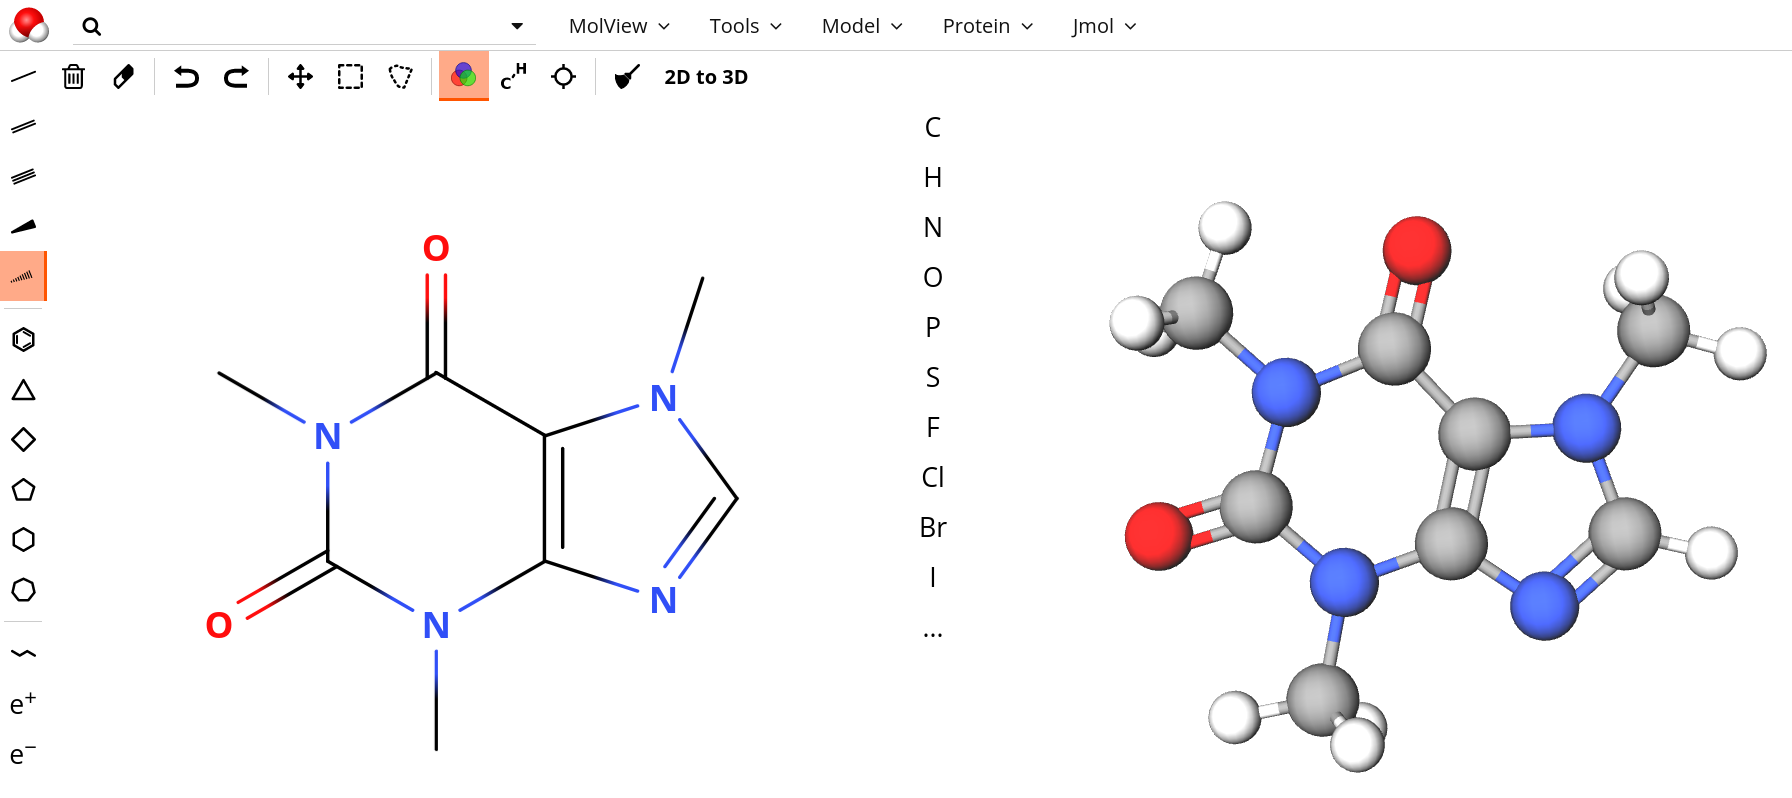
\includegraphics[width=0.9\linewidth]{imgs/bolitasypalitos}
      \caption{Diferentes representaciones de fórmulas estructurales.}
      \label{fig:bolitasypalitos}
    \end{figure}      
  \end{frame}
  %%%%%%%%%%%%%%%%%%%%%%%%%%%%%%%%%%%%%%%%%%%%%%%%%%%%%%%%%%%%
  \section{Estructuras de Lewis y enlaces químicos}
  %%%%%%%%%%%%%%%%%%%%%%%%%%%%%%%%%%%%%%%%%%%%%%%%%%%%%%%%%%%%
  \begin{frame}{¿Qué?}
    Sirve para explicar enlaces y reacciones químicas, de manera simple. Según Lewis, un enlace químico significa compartir o transferir electrones de valencia. Los átomos involucrados obtienen una mayor \emph{estabilidad}.
    \begin{block}{En breve...}
      Cumplir la regla del octeto.
    \end{block}
  \end{frame}
  %%%%%%%%%%%%%%%%%%%%%%%%%%%%%%%%%%%%%%%%%%%%%%%%%%%%%%%%%%%%
  \begin{frame}{¿Por qué?}
    \begin{columns}
      \begin{column}{0.5\textwidth}
        \begin{figure}
          \centering
          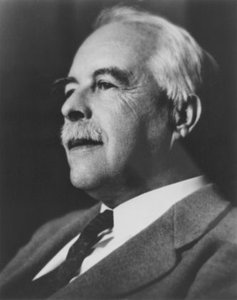
\includegraphics[width=0.7\linewidth]{imgs/Gilbert_N_Lewis}
          \caption{Gilbert N. Lewis}
          \label{fig:gilbertnlewis}
        \end{figure}
      \end{column}
      \begin{column}{0.5\textwidth}
        Ventajas:
        \begin{itemize}
          \item Útil.
          \item Simple.
          \item Química orgánica.
        \end{itemize}
        Desventajas:
        \begin{itemize}
          \item Muy simple.
          \item Tiene algunas excepciones.
        \end{itemize}
      \end{column}
    \end{columns}
  \end{frame}
  %%%%%%%%%%%%%%%%%%%%%%%%%%%%%%%%%%%%%%%%%%%%%%%%%%%%%%%%%%%%
  \begin{frame}{¿Cuándo?}
    \begin{figure}
      \centering
      
\includegraphics[width=1\linewidth]{imgs/Lewis-paper-01}
      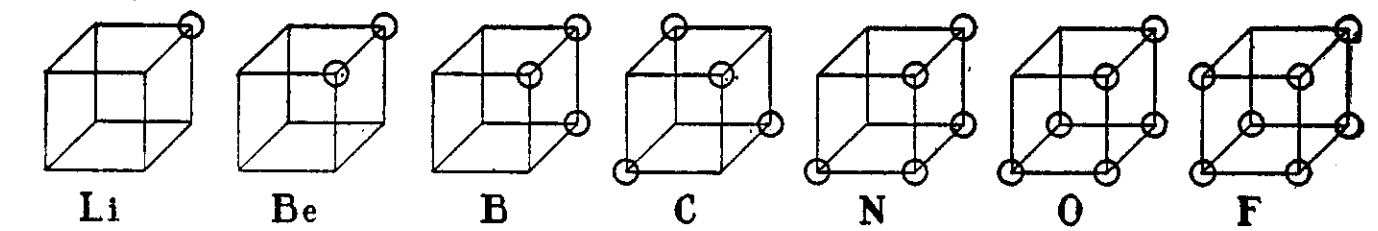
\includegraphics[width=0.7\linewidth]{imgs/Lewis-paper-02}
      \caption{Propone la teoría del átomo cúbico.}
      \label{fig:lewis-paper-01}
    \end{figure}
    Los experimentos \href{https://en.wikipedia.org/wiki/Geiger-Marsden_experiments}{Geiger-Marsden}, dirigidos por Rutherford, tuvieron lugar en 1908-1913. Lewis llevaba haciendo dibujos de estos unos 14 años antes de publicar su artículo.
  \end{frame}
  %%%%%%%%%%%%%%%%%%%%%%%%%%%%%%%%%%%%%%%%%%%%%%%%%%%%%%%%%%%%
  \begin{frame}{¿Cómo?}
    Las reglas:
    \begin{enumerate}
      \item Escribir el esqueleto de la fórmula estructural.
      \item Contar el número de electrones de valencia de los átomos.
      \item Distribuir los electrones entre los átomos enlazantes, de acuerdo a la regla del octeto.
      \item Si no sale, crear enlaces dobles o triples.
    \end{enumerate}
  \end{frame}
  %%%%%%%%%%%%%%%%%%%%%%%%%%%%%%%%%%%%%%%%%%%%%%%%%%%%%%%%%%%%
  \begin{frame}{Enlace iónico}
    % La fuerza electrostática 
    \centering
    Antes...\\
    \bohr{11}{Na} \quad\quad \bohr{17}{Cl}\\
    Después...\\
    \setbohr{atom-style={\footnotesize\sffamily\ch}}
    \bohr{10}{Na+} \bohr{18}{Cl-}
  \end{frame}
  \begin{frame}{Ejemplos: compuestos iónicos}
    \begin{align*}
      \schemestart
      \chemname{\chemfig{\charge{0:1pt=\.}{Li}}}{\scriptsize\elconf{Li}}
      \+
      \chemname{\chemfig{\charge{0:1pt=\.,90:1pt=\:,180:1pt=\:,270:1pt=\:}{F}}}{\scriptsize\elconf{F}}
      \arrow(.mid east--.mid west){->[][][0.8pt]}[,1]
      \schemestop
      &
      \schemestart
      \chemname{\chemfig{\charge{45:2pt=\scriptsize$\oplus$}{Li}\quad\charge{0:1pt=\:,45:2pt=\scriptsize$\ominus$,90:1pt=\:,180:1pt=\:,270:1pt=\:}{F}}}{\scriptsize[\writeelconf{2}]\,\scriptsize[\writeelconf{2,2+6}]}
      \schemestop
      \\[2ex]
      \schemestart
      \chemname{\chemfig{\charge{0:1pt=\.}{Na}}}{\scriptsize\elconf{Na}}
      \+
      \chemname{\chemfig{\charge{0:1pt=\.,90:1pt=\:,180:1pt=\:,270:1pt=\:}{Cl}}}{\scriptsize\elconf{Cl}}
      \arrow(.mid east--.mid west){->[][][0.8pt]}[,1]
      \schemestop
      &
      \schemestart
      \chemname{\chemfig{\charge{45:2pt=\scriptsize$\oplus$}{Na}\quad\charge{0:1pt=\:,45:2pt=\scriptsize$\ominus$,90:1pt=\:,180:1pt=\:,270:1pt=\:}{Cl}}}{\scriptsize[\writeelconf{2,2+6}]\,\scriptsize[\writeelconf{2,2+6,2+6}]}
      \schemestop
      \\[2ex]
      \schemestart
      \chemname{\chemfig{\charge{0:1pt=\.,180:1pt=\.}{Mg}}}{\scriptsize\elconf{Mg}}
      \+
      \chemname{\chemfig{\charge{0:1pt=\:,90:1pt=\:,180:1pt=\.,270:1pt=\.}{O}}}{\scriptsize\elconf{O}}
      \arrow(.mid east--.mid west){->[][][0.8pt]}[,1]
      \schemestop
      &
      \schemestart
      \chemname{\chemfig{\charge{45:2pt=\scriptsize$2\oplus$}{Mg}\quad\charge{0:1pt=\:,45:4pt=\scriptsize$2\ominus$,90:1pt=\:,180:1pt=\:,270:1pt=\:}{O}}}{\scriptsize[\writeelconf{2,2+6}]\,\scriptsize[\writeelconf{2,2+6}]}
      \schemestop
    \end{align*}
    Usualmente este tipo de enlace se da entre un metal y un no metal.
  \end{frame}
  %%%%%%%%%%%%%%%%%%%%%%%%%%%%%%%%%%%%%%%%%%%%%%%%%%%%%%%%%%%%
  \begin{frame}{Enlace covalente}
    % Lone pairs..
    \centering
    Antes...\\
    \bohr{1}{H} \quad\quad \bohr{1}{H}\\
    Después...\\
    \bohr{1}{H}
    \begingroup
    \setbohr{electron-options-add={rotate=180}}    
    \bohr{1}{H}
    \endgroup
  \end{frame}
  %%%%%%%%%%%%%%%%%%%%%%%%%%%%%%%%%%%%%%%%%%%%%%%%%%%%%%%%%%%%
  \begin{frame}{Ejemplos: compuestos covalentes}
    \begin{align*}
      \schemestart
      \chemname{\chemfig{\charge{0:1pt=\.}{H}}}{\scriptsize\elconf{H}}
      \+
      \chemname{\chemfig{\charge{0:1pt=\:,90:1pt=\:,180:1pt=\.,270:1pt=\:}{F}}}{\scriptsize\elconf{F}}
      \arrow(.mid east--.mid west){->[][][0.8pt]}[,1]
      \schemestop
      &
      \schemestart
      \chemname{\chemfig{{H}-[,0.3,,,draw=none]}\charge{0:1pt=\:,90:1pt=\:,180:1pt=\:,270:1pt=\:}{F}}{\scriptsize[\writeelconf{2}]\,\scriptsize[\writeelconf{2,2+6}]}
      \schemestop
      \\[2ex]
      \schemestart
      \chemname{\chemfig{\charge{0:1pt=\.}{2H}}}{\scriptsize\elconf{H}}
      \+
      \chemname{\chemfig{\charge{0:1pt=\:,90:1pt=\:,180:1pt=\.,270:1pt=\.}{O}}}{\scriptsize\elconf{O}}
      \arrow(.mid east--.mid west){->[][][0.8pt]}[,1]
      \schemestop
      &
      \schemestart
      \chemname{\chemfig{{H}-[,0.4,,,draw=none]\charge{0:1pt=\:,90:1pt=\:,180:1pt=\:,270:1pt=\:}{O}-[,0.4,,,draw=none]H}}{\scriptsize[\writeelconf{2}]\,\scriptsize[\writeelconf{2,2+6}]\,\scriptsize[\writeelconf{2}]}
      \schemestop
      \\[2ex]
      \schemestart
      \chemname{\chemfig{\charge{0:1pt=\.,90:1pt=\:,180:1pt=\:,270:1pt=\.}{O}}}{\scriptsize\elconf{O}}
      \+
      \chemname{\chemfig{\charge{0:1pt=\:,90:1pt=\:,180:1pt=\.,270:1pt=\.}{O}}}{\scriptsize\elconf{O}}
      \arrow(.mid east--.mid west){->[][][0.8pt]}[,1]
      \schemestop
      &
      \schemestart
      \chemname{\chemfig{\charge{0:1pt=\:,135:1pt=\:,225:1pt=\:}{O}-[,0.4,,,draw=none]}\charge{180:1pt=\:,45:1pt=\:,315:1pt=\:}{O}}{\scriptsize[\writeelconf{2,2+6}]\,\scriptsize[\writeelconf{2,2+6}]}
      \schemestop
    \end{align*}
    Usualmente este tipo de enlace se da entre átomos no metálicos.
  \end{frame}
  %%%%%%%%%%%%%%%%%%%%%%%%%%%%%%%%%%%%%%%%%%%%%%%%%%%%%%%%%%%%
  \begin{frame}{Excepciones}
    % The transition metals, lanthanides, and actinides all have incompletely filled inner shells, and in general we cannot write simple Lewis dot symbols for them.
    Cuando falla la regla del octeto.
    \begin{itemize}
      \item Dos electrones de valencia (la regla del dueto).
      \item Números impares de electrones de valencia.
      \item Más de ocho electrones de valencia (octeto expandido).
    \end{itemize}
    \begin{align*}
      \schemestart
      \chemname{\chemfig{\charge{0:1pt=\.}{H}}}{\scriptsize\elconf{H}}
      \+
      \chemname{\chemfig{\charge{180:1pt=\.}{H}}}{\scriptsize\elconf{H}}
      \arrow(.mid east--.mid west){->[][][0.8pt]}[,1]
      \schemestop
      &
      \schemestart
      \chemname{\chemfig{{H}-[,0.4,,,draw=none]\charge{180:1pt=\:}{H}}}{\scriptsize[\writeelconf{2}]\,\scriptsize[\writeelconf{2}]}
      \schemestop
      \\[2ex]
      \schemestart
      \chemname{\chemfig{\charge{0:1pt=\.,90:1pt=\:,180:1pt=\.,270:1pt=\.}{N}}}{\scriptsize\elconf{N}}
      \+
      \chemname{\chemfig{\charge{0:1pt=\:,90:1pt=\:,180:1pt=\.,270:1pt=\.}{O}}}{\scriptsize\elconf{O}}
      \arrow(.mid east--.mid west){->[][][0.8pt]}[,1]
      \schemestop
      &
      \schemestart
      \chemname{\chemfig{\charge{0:1pt=\:,90:1pt=\:,180:1pt=\.}{N}-[,0.5,,,draw=none]\charge{-45:0pt=\:,45:0pt=\:,180:1pt=\:}{O}}}{\scriptsize[\writeelconf{2,2+5}]\,\scriptsize[\writeelconf{2,2+6}]}
      \schemestop
      \\[2ex]
      \schemestart
      3\,\chemname{\chemfig{\charge{0:1pt=\.}{H}}}{\scriptsize\elconf{H}}
      \+
      \chemname{\chemfig{\charge{0:1pt=\.,90:1pt=\.,180:1pt=\.}{B}}}{\scriptsize\elconf{B}}
      \arrow(.mid east--.mid west){->[][][0.8pt]}[,1]
      \schemestop
      &
      \schemestart
      \chemname{\chemfig{H-[,0.4,,,draw=none]\charge{0:1pt=\:,90:1pt=\:,180:1pt=\:}{B}(-[2,0.4,,,draw=none]H)-[,0.4,,,draw=none]H}}{\scriptsize B:[\writeelconf{2,2+4}]\,\scriptsize H:[\writeelconf{2}]}
      \schemestop
    \end{align*}
  \end{frame}
  %%%%%%%%%%%%%%%%%%%%%%%%%%%%%%%%%%%%%%%%%%%%%%%%%%%%%%%%%%%%
  \begin{frame}{Electronegatividad (I)}
    La capacidad de atraer los electrones de un enlace químico.
    \begin{figure}
      \centering
      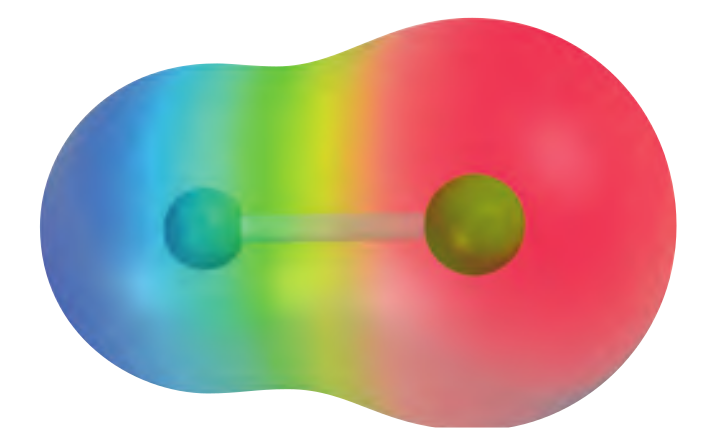
\includegraphics[width=0.8\linewidth]{imgs/emp}
      \caption{Mapa de potencial electrostático de una molécula polar. Fuente: Chemistry, decimocuarta edición, R. Chang \& J. Overby. }
      \label{fig:emp}
    \end{figure}
  \end{frame}
  \begin{frame}{Electronegatividad (II)}
    La diferencia en electronegatividad determina el tipo de enlace.
    \begin{figure}
      \centering
      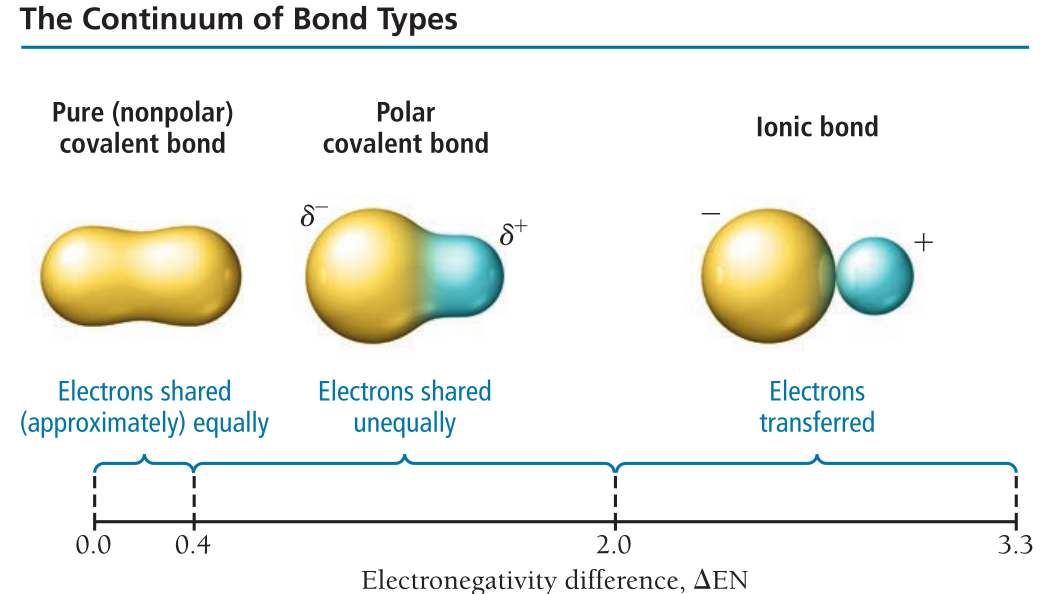
\includegraphics[width=0.9\linewidth]{imgs/polarornonpolar}
      \caption{Fuente: Introductory Chemistry, séptima edición, N. J. Tro.}
      \label{fig:polarornonpolar}
    \end{figure}
  \end{frame}
%%%%%%%%%%%%%%%%%%%%%%%%%%%%%%%%%%%%%%%%%%%%%%%%%%%%%%%%%%%%
\begin{frame}{Tarea:}
  Clasifique cada enlace como covalente, covalente polar o iónico.
  \begin{columns}
    \column{0.5\textwidth}
      \begin{itemize}
      \item \ch{Li-Be}
      \item \ch{Be-O}
      \item \ch{B-C}
      \item \ch{H-F}
      \item \ch{Na-F}
      \end{itemize}
    \column{0.5\textwidth}
    \begin{itemize}
      \item \ch{O-H}
      \item \ch{C-H}
      \item \ch{N-O}
      \item \ch{C-O}
      \item \ch{N-H}
    \end{itemize}
  \end{columns}
Recuerda qué átomos, normalmente, forman un compuesto iónico? Según sus resultados, sucede algo \emph{extraño} con alguno de estos enlaces?
\end{frame}
%%%%%%%%%%%%%%%%%%%%%%%%%%%%%%%%%%%%%%%%%%%%%%%%%%%%%%%%%%%%
\begin{frame}{Propiedades de compuestos iónicos y covalentes}
  %Las fuerzas intermoleculares son débiles, en comparación con los enlaces químicos. Por lo tanto,
  \begin{enumerate}
    \item Los compuestos covalentes son, usualmente, gases, líquidos o sólidos de bajo punto de fusión. 
    %La fuerza electrostática en un compuesto iónico es mucho más fuerte. Por lo tanto 
    \item Los compuestos iónicos son sólidos a temperatura ambiente y tienen puntos de fusión altos.
    \item  A comparación de los compuestos covalentes, la mayoría de los compuestos iónicos se solubilizan en agua y forman soluciones que conducen la electricidad. 
  \end{enumerate}
\end{frame}
%%%%%%%%%%%%%%%%%%%%%%%%%%%%%%%%%%%%%%%%%%%%%%%%%%%%%%%%%%%%
\begin{frame}{Resonancia}
  A veces una estructura de Lewis no es suficiente.
  \begin{align*}
    \schemestart
    \chemfig{\charge{90:1pt=\:,270:1pt=\:}{O}=[,0.6,,,]S(-[2,0.6,,,]\charge{0:1pt=\:,90:1pt=\:,180:1pt=\:}{O})-[,0.6,,,]\charge{0:1pt=\:,90:1pt=\:,270:1pt=\:}{O}}\arrow{<->}\chemfig{\charge{90:1pt=\:,180:1pt=\:,270:1pt=\:}{O}-[,0.6,,,]S(=[2,0.6,,,]\charge{0:1pt=\:,180:1pt=\:}{O})-[,0.6,,,]\charge{90:1pt=\:,270:1pt=\:}{O}}\arrow{<->}
    \chemfig{\charge{90:1pt=\:,180:1pt=\:,270:1pt=\:}{O}-[,0.6,,,]S(-[2,0.6,,,]\charge{0:1pt=\:,90:1pt=\:,180:1pt=\:}{O})=[,0.6,,,]\charge{90:1pt=\:,270:1pt=\:}{O}}
    \schemestop
  \end{align*}
  \begin{block}{Cuidado:}
    Diseñada para tratar las limitaciones de los modelos de Lewis.
  \end{block}
\end{frame}
%%%%%%%%%%%%%%%%%%%%%%%%%%%%%%%%%%%%%%%%%%%%%%%%%%%%%%%%%%%%
\begin{frame}{Tarea:}
  Escriba las estructuras de Lewis y sus estructuras de resonancia, si tiene,  de las siguientes moléculas:
  \begin{itemize}
    \item \ch{H2Se}
    \item \ch{CHCl3}
    \item \ch{BCl3}
    \item \ch{CH3COOH}
    \item \ch{SO2}
    \item \ch{O3}
    \item \ch{NO3}
  \end{itemize}
\end{frame}
%%%%%%%%%%%%%%%%%%%%%%%%%%%%%%%%%%%%%%%%%%%%%%%%%%%%%%%%%%%%
\section{Interacciones no covalentes}
%%%%%%%%%%%%%%%%%%%%%%%%%%%%%%%%%%%%%%%%%%%%%%%%%%%%%%%%%%%%
\begin{frame}{Fuerzas intermoleculares}
  Responsables de las propiedades macroscópicas de la materia. Más débiles que las intramoleculares.
  \begin{itemize}
    \item dispersión
    \item dipolo-dipolo
    \item puente de hidrógeno
    \item ión-dipolo
  \end{itemize}
  %%%%%%%%%%%%%%%%%%%%%%%%%%%%%%%%%%%%%%%%%%%%%%%%%%%%%%%%%%%%
\end{frame}
\begin{frame}{Fuerza de dispersión}
  Mayor nube electrónica, mayor fuerza de dispersión.
  \begin{figure}
    \centering
    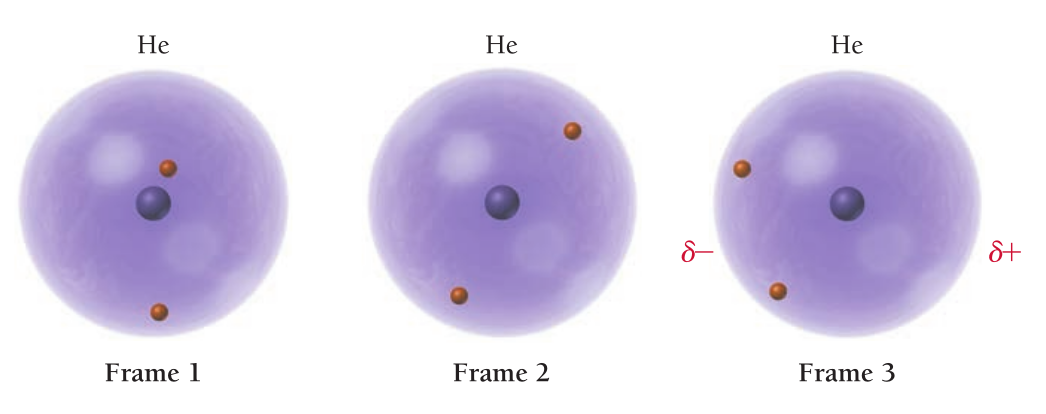
\includegraphics[width=0.7\linewidth]{imgs/dispersionforce01}
    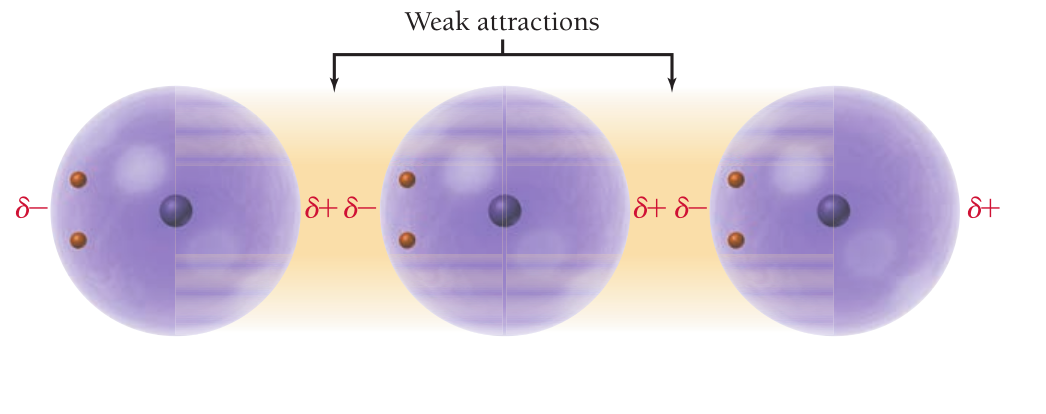
\includegraphics[width=0.7\linewidth]{imgs/dispersionforce02}
    \caption{Un dipolo instantáneo induce dipolos en átomos vecinos. Fuente: Introductory Chemistry, séptima edición, N. J. Tro.}
    \label{fig:dispersionforce01}
  \end{figure}
  % Aparecen y desaparecen
\end{frame}
%%%%%%%%%%%%%%%%%%%%%%%%%%%%%%%%%%%%%%%%%%%%%%%%%%%%%%%%%%%%
\begin{frame}{Fuerza dipolo-dipolo}
  \begin{figure}
    \centering
    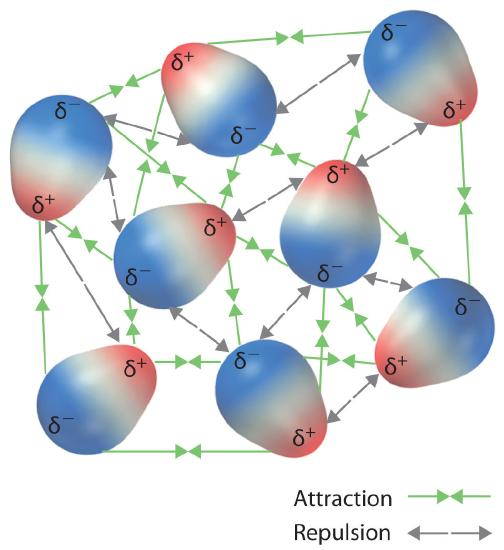
\includegraphics[width=0.55\linewidth]{imgs/dipole-dipole}
    \caption{Moléculas polares tienen dipolos permanentes. Fuente: \href{https://chem.libretexts.org/Courses/Riverland_Community_College}{chem.libretexts.org}.}
    \label{fig:dipoledipole}
  \end{figure}
\end{frame}
%%%%%%%%%%%%%%%%%%%%%%%%%%%%%%%%%%%%%%%%%%%%%%%%%%%%%%%%%%%%
\begin{frame}{Puentes de hidrógeno (I)}
  \begin{figure}
    \centering
    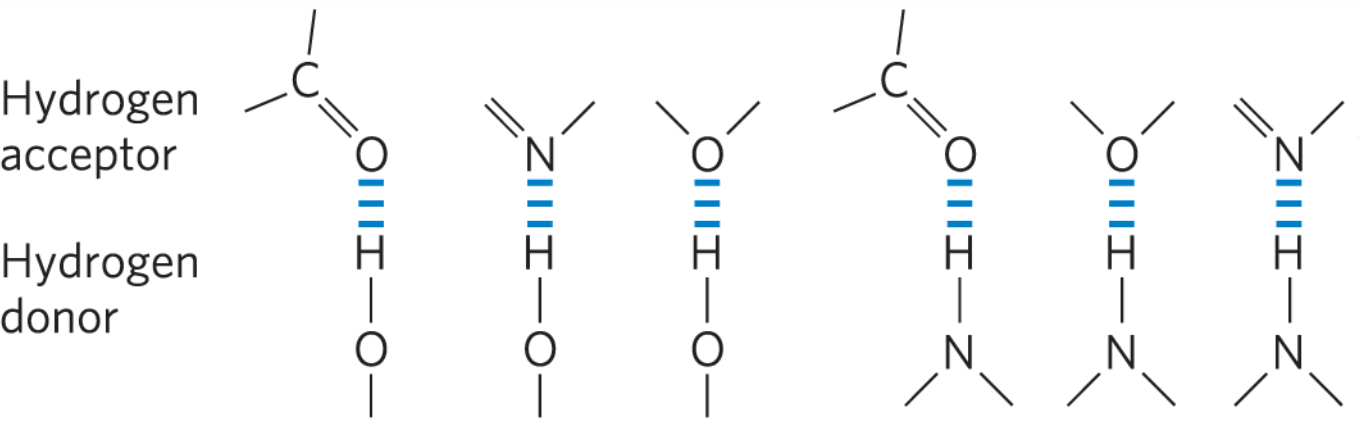
\includegraphics[width=0.7\linewidth]{imgs/hbond-01}
    \caption{Puentes de hidrógeno comunes en sistemas biológicos. Fuente: Principles of Biochemistry, octava edición, D. L. Nelson \& M. M. Cox.}
    \label{fig:hbond-01}
  \end{figure}
\end{frame}
%%%%%%%%%%%%%%%%%%%%%%%%%%%%%%%%%%%%%%%%%%%%%%%%%%%%%%%%%%%%
\begin{frame}{Puentes de hidrógeno (II)}
  \begin{figure}
    \centering
    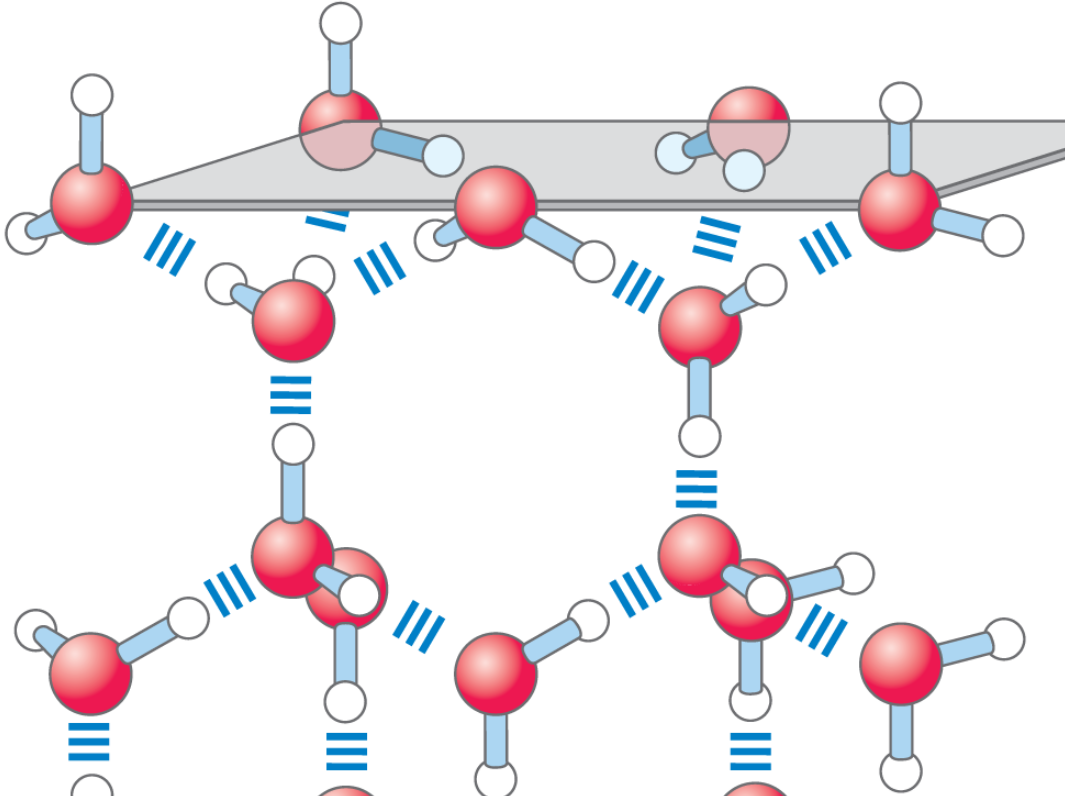
\includegraphics[width=0.7\linewidth]{imgs/hbond}
    \caption{Como un dipolo-dipolo pero más fuerte. Fuente: Principles of Biochemistry, octava edición, D. L. Nelson \& M. M. Cox.}
    \label{fig:hbond}
  \end{figure}
\end{frame}
%%%%%%%%%%%%%%%%%%%%%%%%%%%%%%%%%%%%%%%%%%%%%%%%%%%%%%%%%%%%
\begin{frame}{Ión-dipolo}
  \begin{figure}
    \centering
    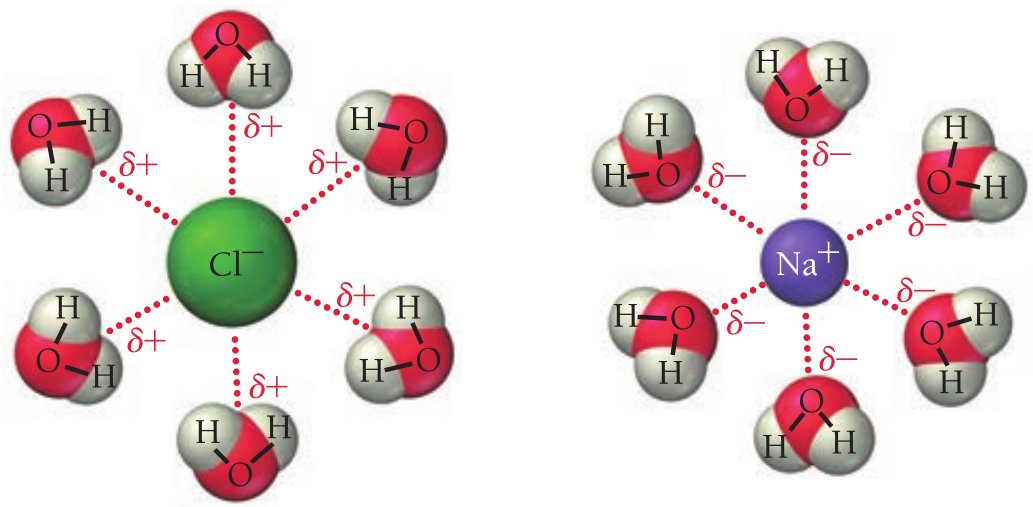
\includegraphics[width=0.7\linewidth]{imgs/ion-dipole}
    \caption{Ocurren en mezclas de compuestos iónicos y compuestos polares. Fuente: Introductory Chemistry, séptima edición, N. J. Tro.}
    \label{fig:ion-dipole}
  \end{figure}
\end{frame}
%%%%%%%%%%%%%%%%%%%%%%%%%%%%%%%%%%%%%%%%%%%%%%%%%%%%%%%%%%%%
\begin{frame}{Resumen}
  \begin{figure}
    \centering
    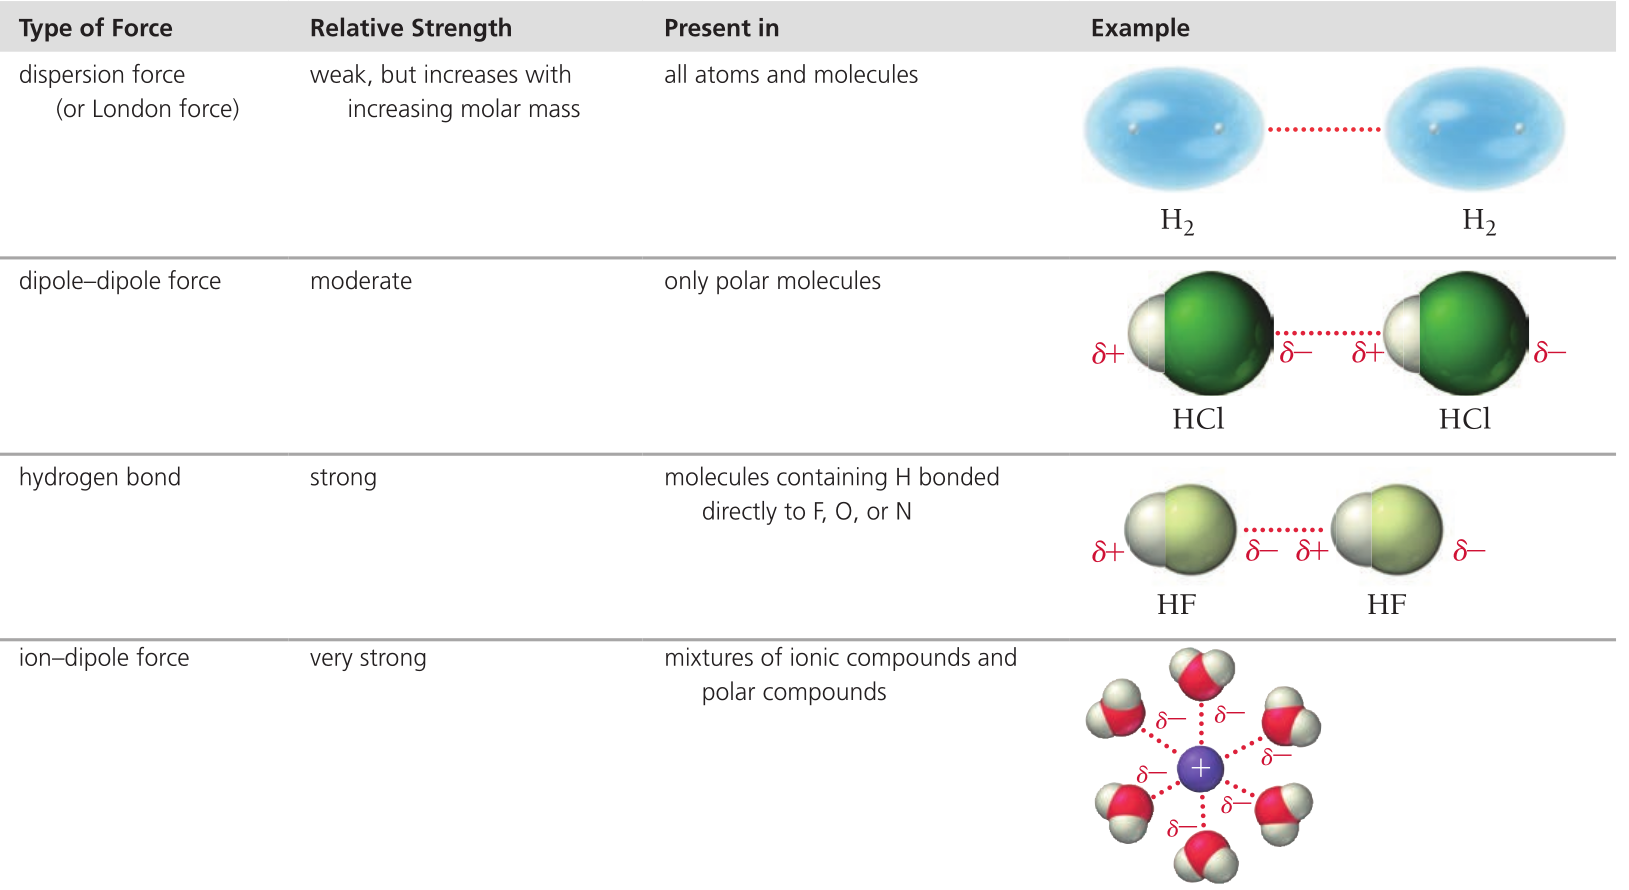
\includegraphics[width=0.95\linewidth]{imgs/summary}
    \caption{Fuente: Introductory Chemistry, séptima edición, N. J. Tro.}
    \label{fig:resumen}
  \end{figure}
\end{frame}
%%%%%%%%%%%%%%%%%%%%%%%%%%%%%%%%%%%%%%%%%%%%%%%%%%%%%%%%%%%%
\begin{frame}{Tarea:}
  \begin{itemize}
    \item Qué molécula tiene el punto de ebullición más alto (\ch{CH2O} o \ch{C2H6}) y por qué?
    \item Qué molécula tiene el punto de ebullición más alto (\ch{CH3OH} o \ch{C2H6}) y por qué?
    \item Qué molécula presentará fuerzas de dipolo-dipolo? (\ch{CO2}, \ch{H2O}, \ch{CH3Cl}, \ch{CH4} y \ch{CCl4})
  \end{itemize}
\end{frame}
%%%%%%%%%%%%%%%%%%%%%%%%%%%%%%%%%%%%%%%%%%%%%%%%%%%%%%%%%%%%
%%%%%%%%%%%%%%%%%%%%%%%%%%%%%%%%%%%%%%%%%%%%%%%%%%%%%%%%%%%%
\begin{frame}{Para leer...}
  Fórmulas químicas:
  \begin{itemize}
    \item \href{https://en.wikipedia.org/wiki/Chemical_formula\#Types}{Tipos de fórmulas químicas}.
  \end{itemize}
  Mol y masa molar:
  \begin{itemize}
    \item \href{https://www.bipm.org/documents/20126/41483022/SI-Brochure-9.pdf}{Mol y masa molar}.
  \end{itemize}
  Estructuras de Lewis
  \begin{itemize}
    \item \href{https://en.wikipedia.org/wiki/History_of_molecular_theory}{Un poco de historia}.
    \item \href{https://en.wikipedia.org/wiki/Gilbert_N._Lewis\#Valence_theory}{Trabajo de Lewis en enlaces químicos}.
    \item \href{https://en.wikipedia.org/wiki/Lewis_structure}{Estructuras de Lewis} (en especial la parte de resonancia y limitaciones).
  \end{itemize}
\end{frame}
%%%%%%%%%%%%%%%%%%%%%%%%%%%%%%%%%%%%%%%%%%%%%%%%%%%%%%%%%%%%
\begin{frame}[standout]{}
  Gracias
\end{frame}
%%%%%%%%%%%%%%%%%%%%%%%%%%%%%%%%%%%%%%%%%%%%%%%%%%%%%%%%%%%%
\end{document}